%%%%%%%%%%%%%%%%%%%%%%%%%%%%%%%%%%%%%%%%%%%%%%%%%%%%%%%%%%%%%%%%%%
% Sample template for MIT Junior Lab Student Written Summaries
% Available from http://web.mit.edu/8.13/www/Samplepaper/sample-paper.tex
%
% Last Updated August 30, 2011
%
% Adapted from the American Physical Societies REVTeK-4.1 Pages
% at http://publish.aps.org
%
% ADVICE TO STUDENTS: Each time you write a paper, start with this
% template and save under a new filename. If convenient, don't
%    erase unneeded lines, just comment them out.  Often, they
%    will be useful containers for information.
%
% Using pdflatex, images must be either PNG, GIF, JPEG or PDF.
%     Turn eps to pdf using epstopdf.
%%%%%%%%%%%%%%%%%%%%%%%%%%%%%%%%%%%%%%%%%%%%%%%%%%%%%%%%%%%%%%%%%%


%%%%%%%%%%%%%%%%%%%%%%%%%%%%%%%%%%%%%%%%%%%%%%%%%%%%%%%%%%%%%%%%%%
% PREAMBLE
% The preamble of a LaTeX document is the set of commands that precede
% the \begin{document} line.  It contains a \documentclass line
% to load the REVTeK-4.1 macro definitions and various \usepackage
% lines to load other macro packages.
%
% ADVICE TO STUDENTS: This preamble contains a suggested set of
% class options to generate a ``Junior Lab'' look and feel that
% facilitate quick review and feedback from one's peers, TA's
% and section instructors. Don't make substantial changes without
%     first consulting your section instructor.
%%%%%%%%%%%%%%%%%%%%%%%%%%%%%%%%%%%%%%%%%%%%%%%%%%%%%%%%%%%%%%%%%%

\documentclass[aps,twocolumn,secnumarabic,balancelastpage,amsmath,amssymb,nofootinbib]{revtex4}
%\documentclass[aps,twocolumn,secnumarabic,balancelastpage,amsmath,amssymb,nofootinbib]{revtex4-1}
\pdfpagewidth 8.5in
\pdfpageheight 11in

%N.B. - Different computers have different packages installed. To compile this template in the current
% Athena environment, REVTeX 4.1 must be used. To use the older REVTeX 4, use the commented out
% Documentclass instead. If you are unable to compile the template at all, you
% may need to update your LaTeX packages. Don't hesitate to speak with your section instructor or a
% TA if you're having issues getting this template to compile.
% Documentclass Options
% aps, prl stand for American Physical Society and Physical Review Letters respectively
    % twocolumn permits two columns, of course
% nobalancelastpage doesn't attempt to equalize the lengths of the two columns on the last page
% as might be desired in a journal where articles follow one another closely
% amsmath and amssymb are necessary for the subequations environment among others
% secnumarabic identifies sections by number to aid electronic review and commentary.
% nofootinbib forces footnotes to occur on the page where they are first referenced
        % and not in the bibliography
% REVTeX 4.1 is a set of macro packages designed to be used withLaTeX 2e.
% REVTeX is well-suited for preparing manuscripts for submissionto APS journals.
       


\usepackage{lgrind} % convert program listings to a form includable in a LaTeX document
\usepackage{chapterbib} % allows a bibliography for each chapter(each labguide has it's own)
\usepackage{color} % produces boxes or entire pages with coloredbackgrounds
\usepackage{graphics}      % standard graphics specifications
\usepackage[pdftex]{graphicx} % alternative graphics specifications
\usepackage{longtable}     % helps with long table options
\usepackage{epsf} % old package handles encapsulated post scriptissues
\usepackage{bm}            % special 'bold-math' package
%\usepackage{asymptote} % For typesetting of mathematical illustrations
\usepackage{thumbpdf}
\usepackage[colorlinks=true]{hyperref} % this package should be added after all others
% use as follows: \url{http://web.mit.edu/8.13}
\usepackage{multirow}
\usepackage{subfigure}

% Define a useful new command for writing units
\newcommand{\cd}{$\cdot$}

%
% And now, begin the document...
%

\begin{document}
\title{Angular Dependence of Cosmic Ray Muon Flux}
\author{Stephen L.\ Eltinge and Jay M.\ Lawhorn}
\email{seltinge@mit.edu; klawhorn@mit.edu}
\date{\today}
\affiliation{MIT Department of Physics}

\begin{abstract}
We propose an experiment to measure the angular dependence of the flux of cosmic ray muons. This experiment expands on the 8.13 cosmic ray muon experiment, which assumes that the flux varies with $\cos^2(\theta)$, where $\theta$ is the incidence angle measured from the vertical. We describe how to test that assumption using a precision scintillator setup provided by Prof.\ Ulrich Becker. \textbf{[Jay, can you add more abstract-appropriate details about your sections here?]}
\end{abstract}

\maketitle

\section{Scientific Motivation}

The interaction of cosmic rays with particles in the upper atmosphere produces showers of muons, charged particles with masses intermediate between those of electrons and protons. These muons travel towards the Earth at near-light speeds; they are able to reach earth due to relativistic time dilation of their lifetime. Because their non-dilated mean lifetime is far too short for them to reach earth, the detection of cosmic ray muons is often used as a simple demonstration of basic relativistic concepts. Cosmic ray muons are also used in high energy physics experiments because they have higher energies than particles that can be produced from particle accelerators.

%\begin{figure}[htb]
%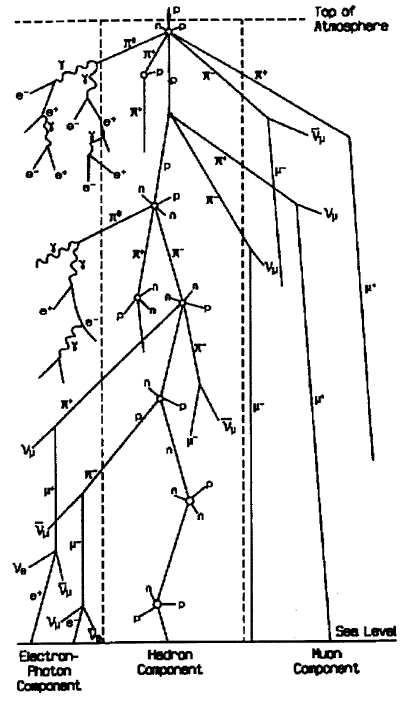
\includegraphics[width=7cm]{muon_shower.png}
%\caption{Figure showing the production of muons and other particles from cosmic rays. Adopted from\cite{grieder}.}
%\label{fig:muon_shower}
%\end{figure}

Figure \ref{fig:muon_shower} shows a schematic of a typical process that produces muons. Cosmic rays, consisting mostly of protons, interact with particles in the upper atmosphere, producing a mixture of elementary particles consisting mostly of pions. These pions decay into a variety of other particles, including the muons that will be detected by our experimental apparatus. In their rest frame, muons have a mean lifetime of about 2.2 $\mu$s and a rest mass of about 105 MeV. In the Earth's frame, cosmic ray muons have a typical energy of around 4 GeV once they reach sea level, indicating that they are moving at highly relativistic speeds.

One experiment in 8.13 finds the velocity of cosmic ray muons via time of flight measurements and their mean lifetime by decay measurements, combining them to conclude that muons must be heavily time dilated. The apparatus in this experiment accepts muons from a variety of incidence angles, and so the analysis requires knowing the angular distribution of incoming muons. 8.13 students generally assume that the distribution follows a $\cos^2(\theta)$ dependence on incident zenith angle, but does not depend on azimuthal angle. This dependence is generally accepted by sources such as \cite{pdg}, but we intend to verify it experimentally.

\section{Hypothesis}

This problem was previously tackled in an undergraduate thesis by MIT student Yi-Hong Kyo.\cite{kuo} Kuo's  thesis cites the following formula for the angular dependence of muon flux:
\begin{equation}
\label{eqn:cosn}
I(\theta,X_h,E)=I(0^\circ)\cos^{n(E,X_h)}(\theta),
\end{equation}
where $X_h$ is the vertical depth and $\Lambda$ is the attenuation length of a particle passing through matter. Like Kuo, we expect to confirm the result that $n(E,X_h)=2$ for the muons that interest us (\emph{i.e.}, those with energies on the order of a few GeV). Kuo also found that the muon flux did not attenuate precisely to zero at angles of $\pm90^\circ$, but rather exhibited small residual ``tails.'' Since our experimental setup will be very similar to his, we anticipate finding this result as well.

\section{Experiment}

\subsection{Apparatus}

We will use a pair of AMS scintillator counters, each of which consists of a long and narrow piece of scintillating material with a triad of photomultiplier tubes (PMT) at each end. We will read out each set of PMTs by oscilliscope.

The scintillation light produced by a muon interacting with the material will propagate and be detected at each end, and the time difference between detection at each end allows reconstruction of the point of interaction. Using a pair of these counters will allow us to reconstruct a flight path for each muon and ultimately an angle of incidence.

\subsection{Method}

We will establish a working bias voltage for the PMTs by measuring the signal frequency as a function of bias voltage. If the bias voltage is too low, we will be losing events that we could otherwise detect. However, if the bias voltage is set too high, our signal will be dominated by amplified noise. We will set bias voltages for each PMT in the plateau between these two regimes.

We will measure the counter detection efficiency by placing two smaller scintillator paddles directly above and below one of the scintillator counters and looking at events where the two smaller paddles register a hit. The percentage of these events in which the middle counter also registers a hit will allow us to calculate the efficiency of the middle counter independently of the efficiencies of the smaller paddles. This setup will also allow us to validate our reconstruction of the point of interaction in the scintillator counter to a certain extent, although the expected precision in point of interaction will likely be much smaller than the additional paddles.

In order to find the angular dependence distribution, we will take data using the four PMT readouts in a series of long integration time runs, and reconstruct the flight path for each detected muon. The angle of incidence with respect to the azimuth can then be calculated. However, we will also need to take into account the geometric acceptance of the pair of scintillator counters, which we will model using a monte carlo simulation. If time permits, we will add detector effects and efficiencies to the simulation using either GEANT4 or a numerical integration scheme.

\section{Expected Results}

We expect to acquire an angular distribution of the incident muons in line with previous measurements going as $\cos^2(\theta)$ with some edge effects. We also expect to make a measurement of the detector efficiency of the scintillator paddles. 

\section{Required Materials}

We will require the pair of AMS scintillator counters, a four-channel USB-capable osciliscope, and if possible, two similarly sized scintillator paddles to be used for efficiency measurements. We hope to borrow the osciliscope from junior lab, and all scintillators from Prof. Becker.

%%%%%%%%%%%%%%%%%%%%%%%%%%%%%%%%%%%%%%%%%%%%%%%%%%%%%%%%%%%%%%%%%%%%%%%%%%%%%
% Place all of the references you used to write this paper in a file
% with the same name as following the \bibliography command
%%%%%%%%%%%%%%%%%%%%%%%%%%%%%%%%%%%%%%%%%%%%%%%%%%%%%%%%%%%%%%%%%%%%%%%%%%%%%

\bibliography{SE_JL_proposal}


\end{document}
